\documentclass{article}
\usepackage[utf8]{inputenc}
\usepackage{multicol}
\usepackage{listings}
\usepackage{verbatim}
\usepackage{color}
\usepackage{geometry}
\usepackage{float}
\usepackage{amsmath}
\usepackage{caption}
\usepackage{pdflscape}
\usepackage{hyperref}
\setlength{\belowcaptionskip}{-10pt}
\setlength{\abovecaptionskip}{-30pt}
\floatstyle{boxed} 
\restylefloat{figure}
\usepackage{graphicx}
\definecolor{codegreen}{rgb}{0,0.6,0}
\definecolor{codegray}{rgb}{0.5,0.5,0.5}
\definecolor{codepurple}{rgb}{0.58,0,0.82}
\definecolor{backcolour}{rgb}{0.95,0.95,0.92}

\lstdefinestyle{mystyle}{
	backgroundcolor=\color{backcolour},   
	commentstyle=\color{codegreen},
	keywordstyle=\color{blue},
	numberstyle=\tiny\color{codegray},
	stringstyle=\color{codepurple},
	basicstyle=\footnotesize,
	breakatwhitespace=false,         
	breaklines=true,                 
	captionpos=b,                    
	keepspaces=true,                 
	numbers=left,                    
	numbersep=5pt,                  
	showspaces=false,                
	showstringspaces=false,
	showtabs=false,                  
	tabsize=2
}

\lstset{style=mystyle}
\title{Data Mining\\
		Home work 08\\Machine Learning Start... }
\author{Aqeel Labash\\ \textbf{Lecturer:} Jaak Vilo}
\date{29 March 2016}

\geometry{
	a4paper,
	total={170mm,257mm},	
	left=10mm,
	top=5mm,
}
\begin{document}
	\maketitle
\section*{First Question}
The quality of classifier as I understood from the page is when we can classify accurately depending on that classifier.By that I mean to have a certain point where it completely separate data into two groups.\\ Another meaning for quality of classifier might be if the classifier really represent a real case or just something happened with high probability in training dataset.If it's just high probability then depending on that classifier will just make our model worst at predicting with real data or unseen data.\\
\section*{Second Question}
For this task I implemented this code in python to get information about the tree.
\begin{lstlisting}[language = Python]
# coding: utf-8
import csv
with open('data.csv') as f:
spam = csv.DictReader(f)
trainset = list(spam)
trainset  = sorted(trainset, key=lambda k: k['Play']) 
len(trainset)
class v:
def __init__(self):
self.lst={}

def AddItem(self,values):

if len(values)<=0:
return
print values[0]
if values[0] in self.lst.keys():
self.lst[values[0]].AddItem(values[1:])
else:
self.lst[values[0]]= v()
self.lst[values[0]].AddItem(values[1:])
def printeverything(self,level=0):
#print 
for itm in self.lst.keys():
thespace = '----'*level
print(thespace+itm)
self.lst[itm].printeverything(level=level+1)
class Core:
def __init__(self,name=None,occurence=0):
self.name = name
self.occurence =occurence
self.sons={}
def AddItem(self,items):
if len(items)<=0:
return
if items[0] in self.sons.keys():
self.sons[items[0]].occurence+=1
self.sons[items[0]].AddItem(items[1:])
else:
self.sons[items[0]] = Core(name=items[0],occurence=1)
self.sons[items[0]].AddItem(items[1:])
def printeverything(self,level=0):
#print 
thespace = '----'*level
print(thespace+str(self.name)+':'+str(self.occurence))
for itm in self.sons.keys():
self.sons[itm].printeverything(level=level+1)
root = Core()
for i in trainset:
root.AddItem((i['Outlook'],i['Temp'],i['Humidity'],i['Windy'],i['Play']))
root.printeverything()
\end{lstlisting}
Which result to the following tree :
\begin{lstlisting}
None:0
----Rainy:5
--------Mild:3
------------High:2
----------------FALSE:1
--------------------Yes:1
----------------TRUE:1
--------------------No:1
------------Normal:1
----------------FALSE:1
--------------------Yes:1
--------Cool:2
------------Normal:2
----------------FALSE:1
--------------------Yes:1
----------------TRUE:1
--------------------No:1
----Overcast:5
--------Hot:2
------------High:1
----------------FALSE:1
--------------------Yes:1
------------Normal:1
----------------FALSE:1
--------------------Yes:1
--------Mild:1
------------High:1
----------------TRUE:1
--------------------Yes:1
--------Cool:2
------------High:1
----------------FALSE:1
--------------------No:1
------------Normal:1
----------------TRUE:1
--------------------Yes:1
----Sunny:5
--------Hot:2
------------High:2
----------------TRUE:1
--------------------No:1
----------------FALSE:1
--------------------No:1
--------Mild:2
------------High:1
----------------FALSE:1
--------------------No:1
------------Normal:1
----------------TRUE:1
--------------------Yes:1
--------Cool:1
------------Normal:1
----------------FALSE:1
--------------------Yes:1
\end{lstlisting}
\textbf{Note:}more clear version available \href{https://github.com/aqeel13932/DM/blob/master/HW08/Q2.ipynb}{here}.Now we have a preview about the data. We choose the levels depending on the entropy by following these steps \href{http://www.saedsayad.com/decision_tree.htm}{(source)} :\\
\begin{enumerate}
	\item First we calculate the \textbf{Entropy} for target: 
	\[E(S) = \sum_{i=1}^{c} -p_i log_2 (p_i)\] 
	\text{in our case we have }
	\[(Yes=9,No=6) \Longrightarrow (Yes =9/15,No = 6/15) \Longrightarrow (Yes =0.6 , No =0.4 ) \]
	\[E(Play Tennis) = E(0.4,0.6) = -0.4*log_2(0.4)-0.6*log_2(0.6)= 0.97095059 \]
	\item Now we calculate the gain for each feature and go greedy to pick which one first.\[Gain(T,X) = E(T)- E(T,X)\]I used the following R code to get the tables : 
	\begin{lstlisting}[language=R]
#### Second Question ######
playing = read.csv('data.csv')
table(playing$Play)
table(playing$Outlook,playing$Play)
table(playing$Temp,playing$Play)
table(playing$Humidity,playing$Play)
table(playing$Windy,playing$Play)
	\end{lstlisting}
	The tables as following :\\
		\begin{tabular}{|l|*{3}{c|}}
			\hline
Outlook \(\backslash\) Play Tennis&No&Yes\\			\hline
Overcast&1&4\\			\hline
Rainy&2&3\\			\hline
Sunny&3&2\\			\hline
		\end{tabular}\\
		Here I explain how to calculate the gain (After that I'll use automate way).
\[Gain = 0.97 - (P(Overcast)*E(1,4)+P(Rainy)*E(2,3)+P(Sunny)*E(3,2))=  \]
\[0.97-(1/3*E(0.2,0.8)+1/3*E(0.4,0.6)+1/3*E(0.6,0.4))\simeq\]
\[0.97-\frac{1}{3}(-0.2*-2.32-0.8*-0.32-0.4*-1.32-0.6*-0.73-0.4*-1.32-0.6*-0.73)= 0.97- 0.884 = 0.086\]
To automate this operation I used the following code:
\begin{lstlisting}[language=R]
#install.packages("entropy")
library(entropy)
#outlook Gain
table(playing$Outlook,playing$Play)
entropy(c(6,9),unit = "log2")-(5/15*entropy(c(1,4),unit = "log2")+5/15*entropy(c(2,3),unit = "log2")+5/15*entropy(c(3,2),unit = "log2"))
#Temp Gain
table(playing$Temp,playing$Play)
entropy(c(6,9),unit = "log2")-(5/15*entropy(c(2,3),unit = "log2")+4/15*entropy(c(2,2),unit = "log2")+6/15*entropy(c(2,4),unit = "log2"))
#Humidity Gain
table(playing$Humidity,playing$Play)
entropy(c(6,9),unit = "log2")-(8/15*entropy(c(5,3),unit = "log2")+7/15*entropy(c(1,6),unit = "log2"))
#Windy Gain
table(playing$Windy,playing$Play)
entropy(c(6,9),unit = "log2")-(9/15*entropy(c(3,6),unit = "log2")+6/15*entropy(c(3,3),unit = "log2"))
\end{lstlisting}
After the previous code is done we have \\
\begin{tabular}{|c|c|} 
\hline
Feature&Gain\\	\hline
OutLook&0.0830075\\	\hline
Temp&0.0133154\\	\hline
Humidity&0.1858052\\	\hline
Windy&0.01997309\\	\hline
\end{tabular}\\
\item From the previous table we can see that the most gain is if we used \textbf{humidity} feature.Now Humidity split our data set into two parts 
(Y=6,N=1 , Humidity = Normal), (Y=3,N=5,Humidity =High).\\
\end{enumerate}
Now we continue to build level two, lets decide the best feature to split when \textbf{humidity is high or Normal.}
\[Eh(PlayTennis)= Eh(5,3)=0.954434,EN(PlayTennis)= EN(1,6)=0.5916728\]
\begin{tabular}{|c|c|c|} 
	\hline
Feature&Humidity=Normal&Humidity=High\\ \hline
OutLook&0.1981174&0.3600731\\	\hline
Temp&0.1280853&0.1100731\\	\hline
Windy&0.1981174&0.003228944\\	\hline
\end{tabular}\\ \\
From previous table we can go with OutLook as my next classifier.In 3rd level, I only did it for 3 groups because while drawing and calculating other groups are already classified.:\\
\begin{tabular}{|c|c|c|c|}
	\hline
&Rainy.Normal&Rainy.High&Overcast.High\\ \hline
Windy&0.9182958&1&0.2516292\\
\hline
Temp&0.2516292&0&0.9182958\\
\hline
\end{tabular}\\
From the previous table we can see that it's best to classify with feature "windy" for branchings (Rainy.Normal,Rainy.High) and with feature "temp" for branch (overcast high).By that no more branches is required as shown in figure 1

\begin{figure}[H]
	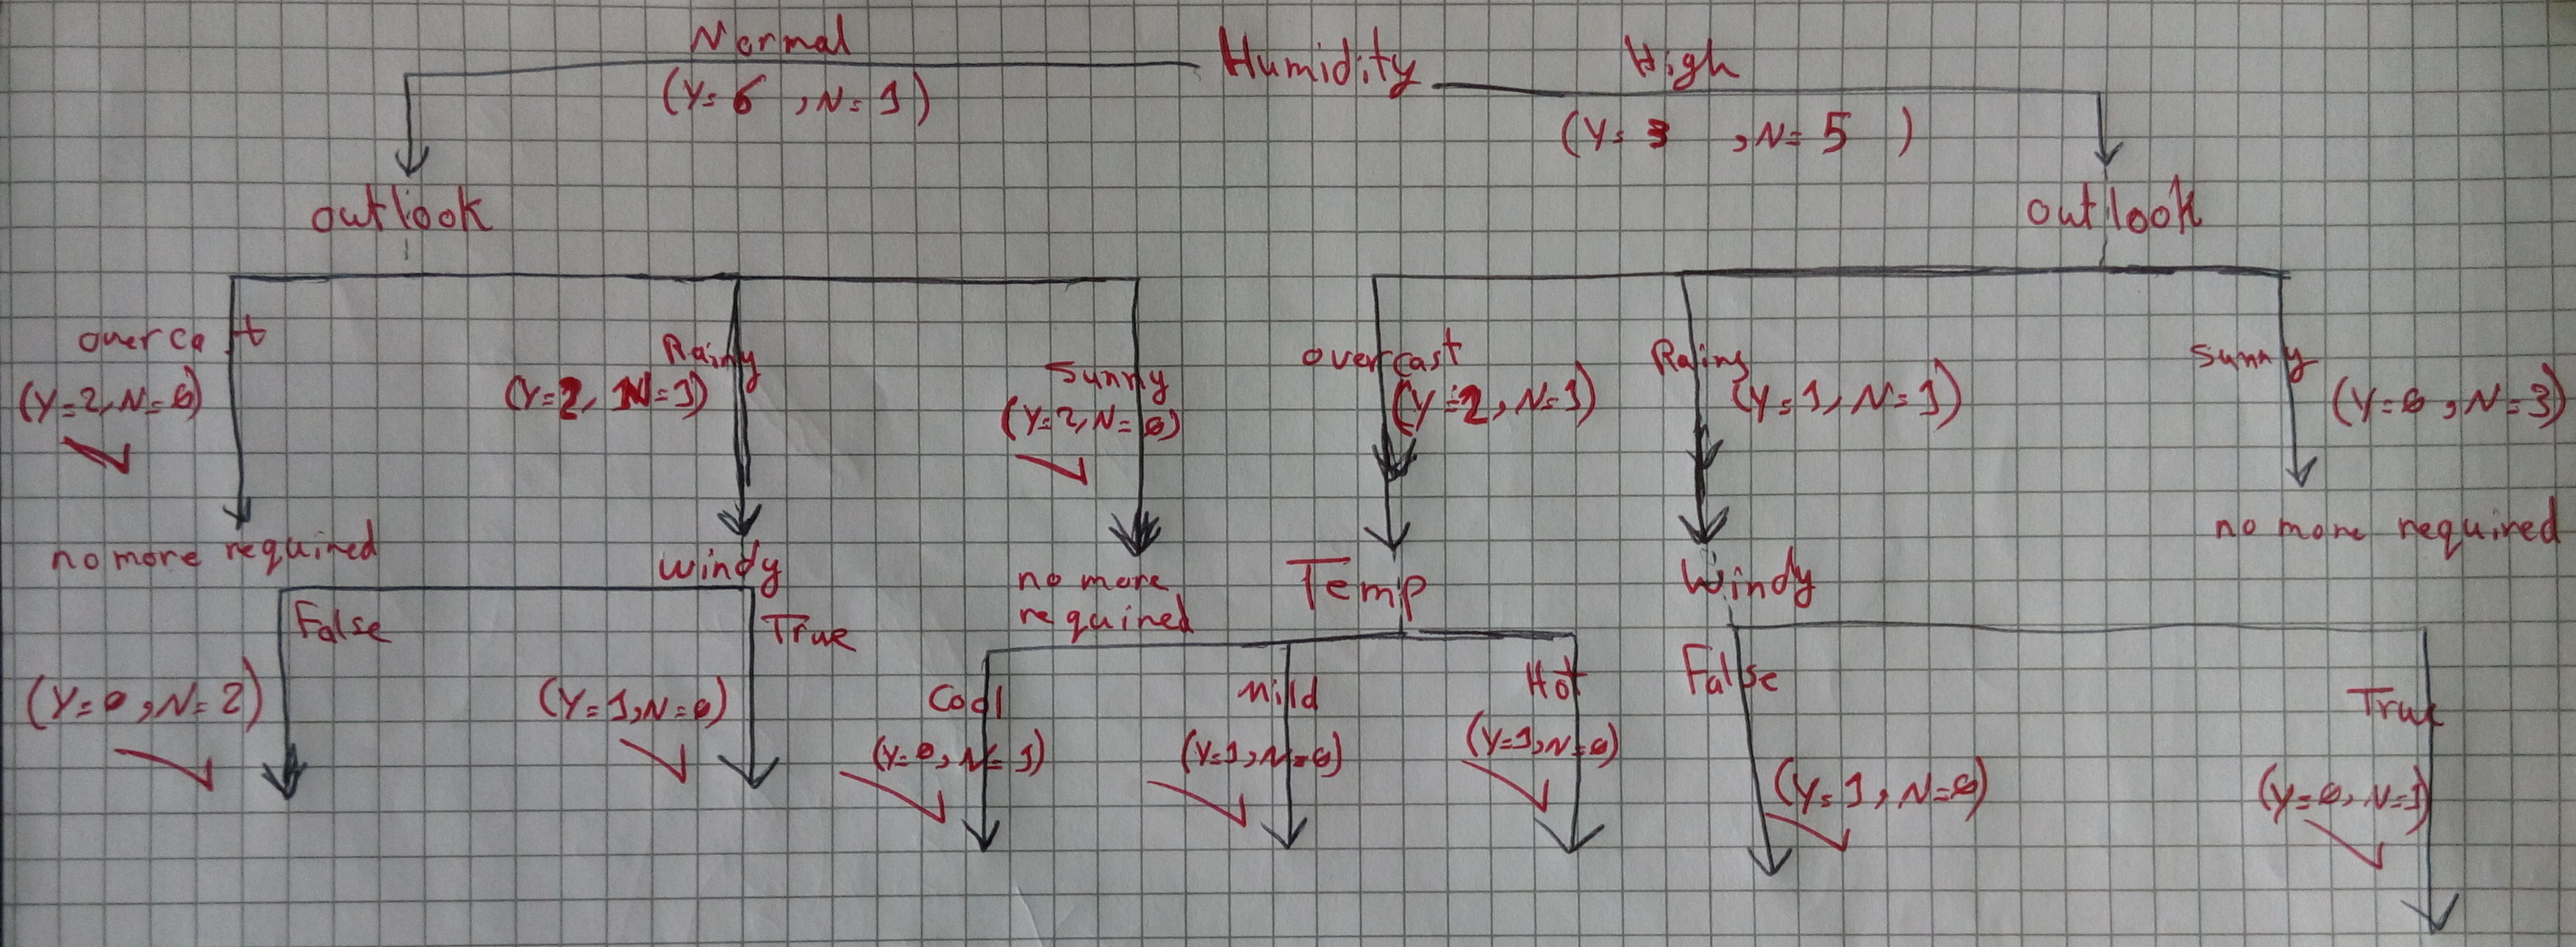
\includegraphics[scale =0.14]{tablecropped.jpg}
	\caption{Decision tree for playing tennis data}
\end{figure}
Following the tree for the scenario (mild, overcast, high humidity and high wind weather) we should play tennis.
The previous calculation done by this code :
\begin{lstlisting}[language=R]
####Level Two####
humidity.h <- subset(playing,playing$Humidity=="High")
humidity.n <- subset(playing,playing$Humidity=="Normal")
#Humidity Normal features gain
#Normal humidity
table(humidity.n$Play)
table(humidity.n$Outlook,humidity.n$Play)
entropy(c(1,6),unit = "log2")-(2/7*entropy(c(0,2),unit = "log2")+3/7*entropy(c(1,2),unit = "log2")+2/7*entropy(c(0,2),unit = "log2"))
table(humidity.n$Temp,humidity.n$Play)
entropy(c(1,6),unit = "log2")-(4/7*entropy(c(1,3),unit = "log2")+1/7*entropy(c(0,1),unit = "log2")+2/7*entropy(c(0,2),unit = "log2"))
table(humidity.n$Windy,humidity.n$Play)
entropy(c(1,6),unit = "log2")-(4/7*entropy(c(0,4),unit = "log2")+3/7*entropy(c(1,2),unit = "log2"))
#High humidity
table(humidity.h$Play)
table(humidity.h$Outlook,humidity.h$Play)
entropy(c(5,3),unit = "log2")-(3/8*entropy(c(1,2),unit = "log2")+2/8*entropy(c(1,1),unit = "log2")+3/8*entropy(c(3,0),unit = "log2"))
table(humidity.h$Temp,humidity.h$Play)
entropy(c(5,3),unit = "log2")-(1/8*entropy(c(1,0),unit = "log2")+3/8*entropy(c(2,1),unit = "log2")+4/8*entropy(c(2,2),unit = "log2"))
table(humidity.h$Windy,humidity.h$Play)
entropy(c(5,3),unit = "log2")-(5/8*entropy(c(3,2),unit = "log2")+3/8*entropy(c(2,1),unit = "log2"))
#### Level 3 #####
table(playing$Outlook)
rainy.normal<- subset(playing,playing$Humidity=="Normal" & playing$Outlook=="Rainy")
rainy.high<- subset(playing,playing$Humidity=="High" & playing$Outlook=="Rainy")
overcast.high<- subset(playing,playing$Humidity=="High" & playing$Outlook=="Overcast")
#Rainy Normal branch
table(rainy.normal$Play)
table(rainy.normal$Windy,rainy.normal$Play)
entropy(c(1,2),unit = "log2")-(2/3*entropy(c(0,2),unit = "log2")+1/3*entropy(c(1,0),unit = "log2"))
table(rainy.normal$Temp,rainy.normal$Play)
entropy(c(1,2),unit = "log2")-(2/3*entropy(c(1,1),unit = "log2")+1/3*entropy(c(0,1),unit = "log2"))
#Rainy High branch
table(rainy.high$Play)
table(rainy.high$Windy,rainy.high$Play)
entropy(c(1,1),unit = "log2")-(1/2*entropy(c(0,1),unit = "log2")+1/2*entropy(c(1,0),unit = "log2"))
table(rainy.high$Temp,rainy.high$Play)
entropy(c(1,1),unit = "log2")-(entropy(c(1,1),unit = "log2"))
#overcast high branch
table(overcast.high$Play)
table(overcast.high$Windy,overcast.high$Play)
entropy(c(1,2),unit = "log2")-(2/3*entropy(c(1,1),unit = "log2")+1/3*entropy(c(0,1),unit = "log2"))
table(overcast.high$Temp,overcast.high$Play)
entropy(c(1,2),unit = "log2")-(1/3*entropy(c(1,0),unit = "log2")+1/3*entropy(c(0,1),unit = "log2")+1/3*entropy(c(0,1),unit = "log2"))
\end{lstlisting}
\section*{Third Question}
For this task I used R with rpart to generate the decision tree, and here is the code :
\begin{lstlisting}[language=R]
png('tree.png',width = 1600,height = 800)
plot(result, uniform=TRUE,
main="Classification Tree for Cars")
text(result, use.n=TRUE, all=TRUE, cex=.8)
dev.off()
\end{lstlisting}
From the previous code we get the following tree :
\begin{landscape}
\begin{figure}[H]
	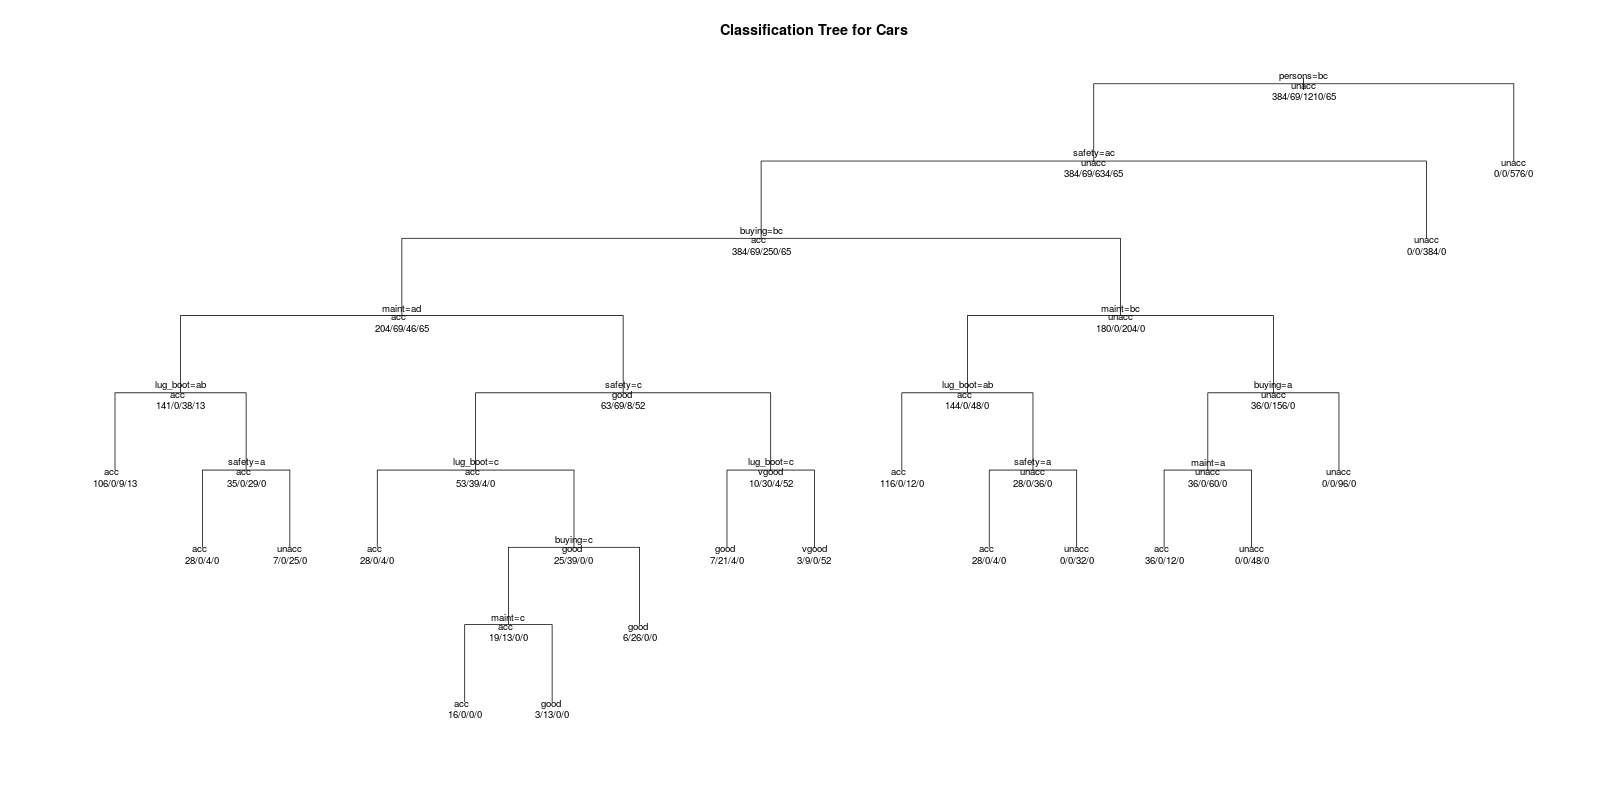
\includegraphics[scale=0.47]{tree.png}
	\caption{Tree of decision tree classification}
\end{figure}
Under each node in the tree we can see 4 numbers which represent the number of objects in each category at the following order (acc,good,unacc,vgood).
After that I used this code to get rules list :
\begin{lstlisting}[language=R]
library(arules)
rules = apriori(cars )
inspect(rules)
\end{lstlisting}
\end{landscape}
\begin{tabular}{|l|*{6}{c|}}
	\hline
&lhs&rhs&support&confidence&lift\\
\hline
1&{buying=vhigh}&{acceptability=unacc}&0.2083333&0.8333333&1.190083\\
\hline
2&{maint=vhigh}&{acceptability=unacc}&0.2083333&0.8333333&1.190083\\\hline
3&{safety=low}&{acceptability=unacc}&0.3333333&1.0&1.428099\\\hline
4&{persons=2}&{acceptability=unacc}&0.3333333&1.0&1.428099\\\hline
5&{lug\_boot=big,safety=low}&{acceptability=unacc}&0.1111111&1.0&1.428099\\\hline
6&{persons=2,lug\_boot=big}&{acceptability=unacc}&0.1111111&1.0&1.428099\\\hline
7&{persons=4,safety=low}&{acceptability=unacc}&0.1111111&1.0&1.428099\\\hline
8&{persons=more,safety=low}&{acceptability=unacc}&0.1111111&1.0&1.428099\\\hline
9&{lug\_boot=med,safety=low}&{acceptability=unacc}&0.1111111&1.0&1.428099\\\hline
10&{persons=2,lug\_boot=med}&{acceptability=unacc}&0.1111111&1.0&1.428099\\\hline
11&{persons=2,safety=high}&{acceptability=unacc}&0.1111111&1.0&1.428099\\\hline
12&{persons=2,safety=med}&{acceptability=unacc}&0.1111111&1.0&1.428099\\\hline
13&{lug\_boot=small,safety=low}&{acceptability=unacc}&0.1111111&1.0&1.428099\\\hline
14&{persons=2,safety=low}&{acceptability=unacc}&0.1111111&1.0&1.428099\\\hline
15&{persons=2,lug\_boot=small}&{acceptability=unacc}&0.1111111&1.0&1.428099\\\hline
\end{tabular}\\
For comparison I think the association rules some how looks like sub category of decision tree.Because we can recreate the tree as an association rules.Another thing, I think build a tree of association rules may help as well in shortening the rules number. In the rules table row 4 is the right branch of the root node in the tree.
\section*{Fourth Question}
We already find the decision tree in the third question, but to find Naive Bayes I used the following code :
\begin{lstlisting}[language=R]
########### Fourth Question #############
#install.packages("klaR")
library(klaR)
nbayestree<- NaiveBayes(acceptability~.,data = cars)
summary(nbayestree)
nbayestree$tables$buying
nbayestree$tables$maint
nbayestree$tables$doors
nbayestree$tables$persons
nbayestree$tables$lug_boot
nbayestree$tables$safety
\end{lstlisting}
Using the previous tool generate 6 tables, each table has the acceptability as rows and categories as columns and the table filled with probabilities.Here is the tables :\\
Acceptability  probability with buying categories\\
\begin{tabular}{|l|*{5}{c|}}
	\hline
	grouping&high&low&med&vhigh\\ \hline
	acc&0.2812500&0.2317708&0.2994792&0.1875000 \\ \hline
	good&0.0000000&0.6666667&0.3333333&0.0000000\\ \hline
	unacc&0.2677686&0.2132231&0.2214876&0.2975207\\ \hline
	vgood&0.0000000&0.6000000&0.4000000&0.0000000\\ \hline
\end{tabular}
\\\\Acceptability  probability with maint categories\\
\begin{tabular}{|l|*{5}{c|}}
\hline
grouping&high&low&med&vhigh\\ \hline
acc&0.2734375&0.2395833&0.2994792&0.1875000\\ \hline
good&0.0000000&0.6666667&0.3333333&0.0000000\\ \hline
unacc&0.2595041&0.2214876&0.2214876&0.2975207\\ \hline
vgood&0.2000000&0.4000000&0.4000000&0.0000000\\ \hline
\end{tabular}
\\\\Acceptability  probability with doors categories\\
\begin{tabular}{|l|*{5}{c|}}
	\hline
grouping&2&3&4&5more\\ \hline
acc&0.2109375&0.2578125&0.2656250&0.2656250\\ \hline
good&0.2173913&0.2608696&0.2608696&0.2608696\\ \hline
unacc&0.2694215&0.2479339&0.2413223&0.2413223\\ \hline
vgood&0.1538462&0.2307692&0.3076923&0.3076923\\ \hline
\end{tabular}
\\\\Acceptability  probability with persons categories\\
\begin{tabular}{|l|*{4}{c|}}
	\hline
	grouping&2&4&more\\ \hline
acc&0.0000000&0.5156250&0.4843750\\ \hline
good&0.0000000&0.5217391&0.4782609\\ \hline
unacc&0.4760331&0.2578512&0.2661157\\ \hline
vgood&0.0000000&0.4615385&0.5384615\\ \hline
\end{tabular}
\\\\Acceptability  probability with lug\_boot categories\\
\begin{tabular}{|l|*{4}{c|}}
	\hline
	grouping&big&med&small\\ \hline
acc&0.3750000&0.3515625&0.2734375\\ \hline
good&0.3478261&0.3478261&0.3043478\\ \hline
unacc&0.3041322&0.3239669&0.3719008\\ \hline
vgood&0.6153846&0.3846154&0.0000000\\ \hline
\end{tabular}
\\\\Acceptability  probability with safety categories\\
\begin{tabular}{|l|*{4}{c|}}
	\hline
	grouping&high&low&med\\ \hline
acc&0.5312500&0.0000000&0.4687500\\ \hline
good&0.4347826&0.0000000&0.5652174\\ \hline
unacc&0.2289256&0.4760331&0.2950413\\ \hline
vgood&1.0000000&0.0000000&0.0000000\\ \hline
\end{tabular}\\ \\
Up to this point to be able to judge maybe it'll need a long staring at those table, but  I think to be able to judge for real is to put the models to the test and check which one predict better with higher accuracy.\\
Now for 10 folds I'll divide the data 90 \%for training-10 \% for testing.To be able to compare Naive Bayes with decision tree I'll use the same data for both (first pick them randomly then use them).Here is the code I used for this task :
\begin{lstlisting}[language=R]
##Testing.
#install.packages("ROCR")
#install.packages("getopt")
library(gplots)
library(ROCR)
library(e1071)
library(getopt)
library(rpart)
Compare<-function()
{
bcmVector<- (c(OverallAccuracy=0,recallAcc=0,recallGood=0,recallunacc=0,recallVgood=0,precisionAcc=0,
precisionGood=0,precisionunacc=0,precisionVgood=0))
dtcmVector<- (c(OverallAccuracy=0,recallAcc=0,recallGood=0,recallunacc=0,recallVgood=0,precisionAcc=0,
precisionGood=0,precisionunacc=0,precisionVgood=0))
for(i in seq_len(10))
{
# 1728 * 0.9 ~ 1556 , 1728*0.1~172
#Shuffle the list To use it later
tmp<-cars[sample(nrow(cars)),]
nbp<-predict(NaiveBayes(acceptability~.,data = tmp[c(1:1556),]),tmp[c(1557:1728),])
dtreep<-predict(rpart(acceptability~.,data = tmp[c(1:1556),]),newdata =  tmp[c(1557:1728),],type = 'class')
bcm<-table(nbp$class,tmp[c(1557:1728),]$acceptability)
dtcm<-table(dtreep,tmp[c(1557:1728),]$acceptability)
#print (bcm)
bcmVector<-bcmVector +c(OverallAccuracy=sum(diag(bcm))/sum(bcm),recallAcc=bcm[1,1]/sum(bcm[1,]),
recallGood=bcm[2,2]/sum(bcm[2,]),recallunacc=bcm[3,3]/sum(bcm[3,]),
recallVgood=bcm[4,4]/sum(bcm[4,]),precisionAcc=bcm[1,1]/sum(bcm[,1]),
precisionGood=bcm[2,2]/sum(bcm[,2]),precisionunacc=bcm[3,3]/sum(bcm[,3]),
precisionVgood=bcm[4,4]/sum(bcm[,4]))
#print (dtcm)
dtcmVector<-dtcmVector+c(OverallAccuracy=sum(diag(dtcm))/sum(dtcm),recallAcc=dtcm[1,1]/sum(dtcm[1,]),
recallGood=dtcm[2,2]/sum(dtcm[2,]),recallunacc=dtcm[3,3]/sum(dtcm[3,]),
recallVgood=dtcm[4,4]/sum(dtcm[4,]),precisionAcc=dtcm[1,1]/sum(dtcm[,1]),
precisionGood=dtcm[2,2]/sum(dtcm[,2]),precisionunacc=dtcm[3,3]/sum(dtcm[,3]),
precisionVgood=dtcm[4,4]/sum(dtcm[,4]))
}
print(bcmVector/10)
print (dtcmVector/10)
}
\end{lstlisting}
The result would for confusion matrix will look like this :\\ 
\begin{tabular}{|l|*{5}{c|}}
	\hline
&acc&good&unacc&vgood\\
\hline
acc&26&4&5&4\\ \hline
good&2&3&1&0\\ \hline
unacc&9&0&114&0\\ \hline
vgood&0&1&0&3\\ \hline
\end{tabular}\\
\begin{landscape}
(I just put a real example of output data , didn't think that we have to put the output for 10 X 2, folds X ways(Naive Bayes,Decision Tree))
As a reminder \[Accuracy = \frac{TP+TN}{Totall},Precision = \frac{TP}{TP+FP},Recall = \frac{TP}{TP+FN}\] 
The previous function will output the average measurements for 10 folds for Naive Bayes , decision tree table. and the output as following :\\
Naive Bayes \\
\begin{tabular}{|l|*{9}{c|}}
		\hline
	Accuracy&recallAcc&recallGood&recallunacc&recallVgood&precisionAcc&precisionGood&precisionunacc&precisionVgood\\ 		\hline
0.8581395&0.6705130&0.6916667&0.9178775&NaN&0.6936558&0.3139791&0.9592180&0.5475000 \\		\hline
\end{tabular}\\

Decision tree model\\
\begin{tabular}{|l|*{9}{c|}}
	\hline
	OverallAccuracy&recallAcc&recallGood&recallunacc&recallVgood&precisionAcc&precisionGood&precisionunacc&precisionVgood\\ \hline
0.9366279&0.8489693&0.7262748&0.9881618&0.7643146&0.8967532&0.8830556&0.9577577&0.7975000\\ \hline
\end{tabular}\\
From the previous two tables now I can say that in our case the decision tree is better model than Naive Bayes for  this data.
\end{landscape}
\section*{Fifth Question}
For this question I used the following code in R : 
\begin{lstlisting}[language=R]
############## 5th Question #############
rm(list=ls())
setwd('/home/aqeel/Study/DM/HW08/')
titanic <- read.csv('titanic.txt')
library(klaR)
library(gplots)
library(ROCR)
library(arules)
library(rpart)
#Shuffle the list To use it later
tmp<-titanic[sample(nrow(titanic)),]
nbmodel<-NaiveBayes(Survived~.,data = tmp[c(1:1981),])
print(nbmodel$tables)
dtmodel<-rpart(Survived~.,data = tmp[c(1:1981),])
png('treetitanic.png',width = 1600,height = 800)
plot(dtmodel, uniform=TRUE,
main="Classification Tree for Titanic survivres")
text(dtmodel, use.n=TRUE, all=TRUE, cex=.8)
dev.off()

therules<- apriori(tmp[c(1:1981),],parameter = list(supp=0.05,conf=0.7),
appearance = list(rhs=c("Survived=Yes","Survived=No"),default="lhs"))
print (inspect(therules))
\end{lstlisting}
From the previous code we get the following tables :\\
\begin{tabular}{|l|*{6}{c|}}
	\hline
	&lhs&rhs&support&confidence&lift\\ \hline
1&{Sex=Female}&{Survived=Yes}&0.15648662&0.7434053&2.272663\\ \hline
2&{Class=3rd}&{Survived=No}&0.23220596&0.7419355&1.102606\\ \hline
3&{Class=Crew}&{Survived=No}&0.30792529&0.7540173&1.120561\\ \hline
4&{Sex=Male}&{Survived=No}&0.61887935&0.7838875&1.164952\\ \hline
5&{Class=2nd,Sex=Male}&{Survived=No}&0.07016658&0.8633540&1.283049\\ \hline
6&{Class=1st,Sex=Female}&{Survived=Yes}&0.06208985&0.9685039&2.960812\\ \hline
7&{Sex=Female,Age=Adult}&{Survived=Yes}&0.14336194&0.7513228&2.296868\\ \hline
8&{Class=3rd,Sex=Male}&{Survived=No}&0.18727915&0.8244444&1.225225\\ \hline
9&{Class=3rd,Age=Adult}&{Survived=No}&0.21100454&0.7572464&1.125360\\ \hline
10&{Class=Crew,Sex=Male}&{Survived=No}&0.30742049&0.7728426&1.148538\\ \hline
11&{Class=Crew,Age=Adult}&{Survived=No}&0.30792529&0.7540173&1.120561\\ \hline
12&{Sex=Male,Age=Adult}&{Survived=No}&0.60424028&0.7937666&1.179634\\ \hline
13&{Class=2nd,Sex=Male,Age=Adult}&{Survived=No}&0.07016658&0.9144737&1.359019\\ \hline
14&{Class=1st,Sex=Female,Age=Adult}&{Survived=Yes}&0.06208985&0.9685039&2.960812\\ \hline
15&{Class=3rd,Sex=Male,Age=Adult}&{Survived=No}&0.17264008&0.8382353&1.245720\\ \hline
16&{Class=Crew,Sex=Male,Age=Adult}&{Survived=No}&0.30742049&0.7728426&1.148538\\ \hline
\end{tabular}\\ \\ 
\begin{lstlisting}
$Class
var
grouping        1st       2nd       3rd      Crew
No  0.08177044 0.1065266 0.3555889 0.4561140
Yes 0.29320988 0.1620370 0.2546296 0.2901235

$Sex
var
grouping     Female      Male
No  0.08627157 0.9137284
Yes 0.48765432 0.5123457

$Age
var
grouping     Adult      Child
No  0.9639910 0.03600900
Yes 0.9228395 0.07716049
\end{lstlisting}
\begin{figure}[H]
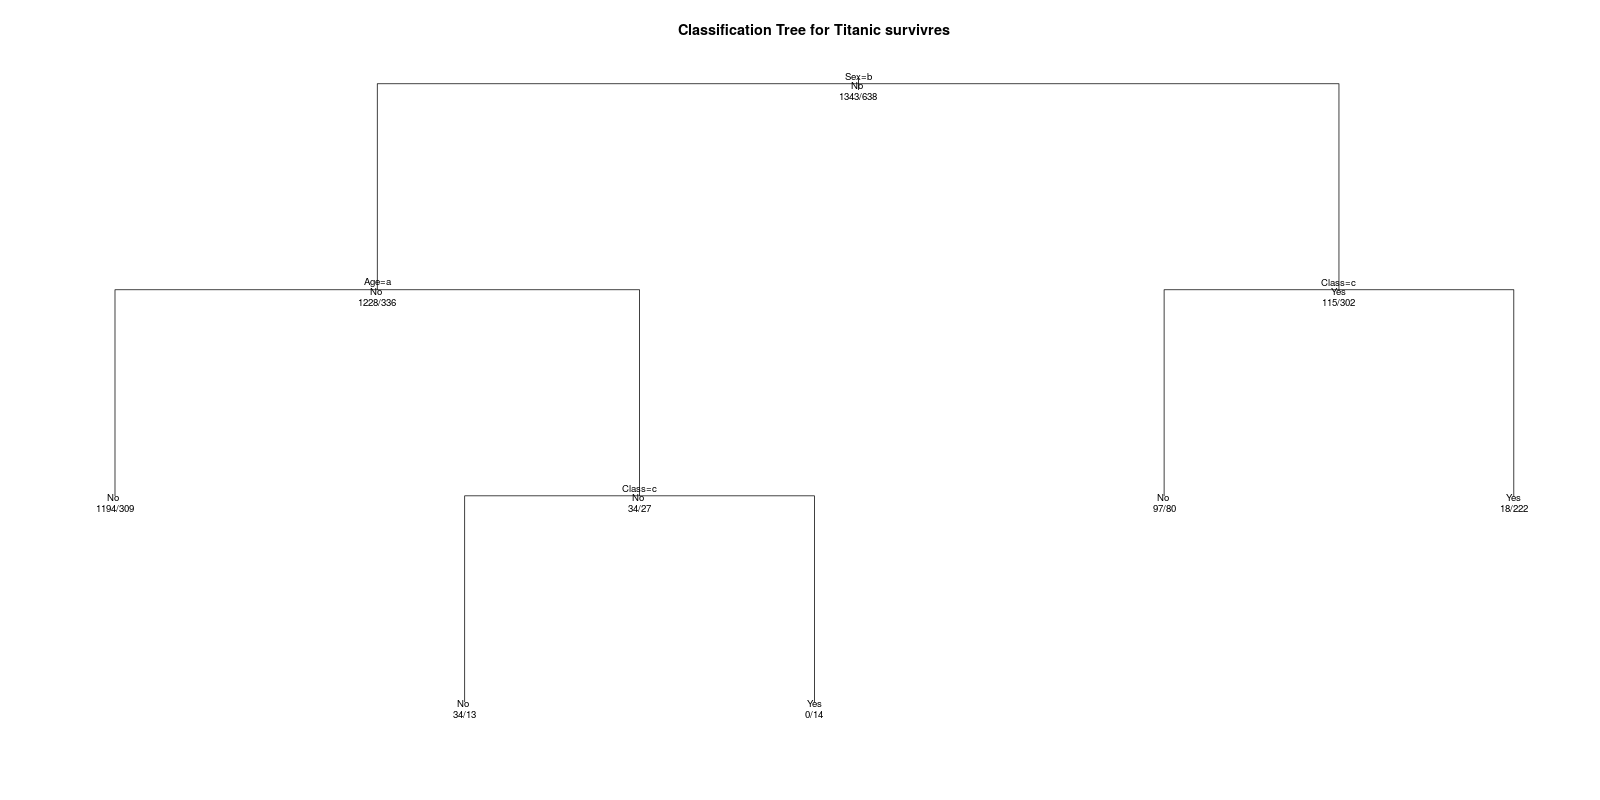
\includegraphics[scale=0.3]{treetitanic.png}
\caption{Shows the decision tree for titanic 0.9 of the data1}
\end{figure}
From the previous tables and figures we can notice for example if we have the following :
Crew,Adult,Male. All previous method will classify as not survived.\\ Actually I tried many example for for this data they reach to the same decision.\\
To characterize and interpret those methods : I think decision tree with the long use it might get stuck and talk long time to change. While naive Bayes will change by each record (enhance the probabilities values).I think apriori algorithm some how close to decision table and it'll take long time to converge in case changes happened in the environment. 
\section*{Sixth Question}
To minimize over fitting there is many ways.
\begin{enumerate}
	\item Add noise layer so we can decrease the over fitting.\href{http://keras.io/layers/noise/}{source}
	\item Use different data for training and test each time.
	\item Idea: we train the model till the moment where the train accuracy increase and the test accuracy decreased.
\end{enumerate}
I used the Connect4 dataset , I trained it on 80 \% and tested on 20\%. I used this code to generate the confusion matrix :
\begin{lstlisting}[language=R]
########### Sixth Question ##########
rm(list=ls())
connect4<-read.csv('connect-4.data',header = FALSE,sep = ",")
colnames(connect4)<-c('a1','a2','a3','a4','a5','a6','b1','b2','b3','b4','b5','b6','c1','c2','c3','c4','c5','c6','d1','d2','d3','d4','d5','d6','e1','e2','e3','e4','e5','e6','f1','f2','f3','f4','f5','f6','g1','g2','g3','g4','g5','g6','result')

##Over fitting example ##
connect4<-connect4[sample(nrow(connect4)),]
# 67557*0.8 ~ 54046 , 67557*0.2~13511
nbmodel<-NaiveBayes(result~.,connect4[c(0:54046),])
nbp<-predict(nbmodel,connect4[c(54047:67557),])
table(nbp$class,connect4[c(54047:67557),]$result)
\end{lstlisting}
And here is the confusion matrix.
\begin{tabular}{|c|c|c|c|}
\hline
&draw&loss&win \\ \hline
draw&88&112&143\\ \hline
loss&157&1372&443\\ \hline
win&1079&1778&8339\\ \hline
\end{tabular}
The previous table Over all Accuracy was 0.7252609 , where the cars dataset over all accuracy was : 0.8581395.\\
\text{Note:}All R,python,ipython,tex,pdf,etc.. files exist on \href{https://github.com/aqeel13932/DM/tree/master/HW08}{github}
\begin{center}
\textbf{ E.O.F}
\end{center}
\end{document}